\providecommand{\Fun}{\operatorname{Fun}}
\providecommand{\QCat}{\mathcal{Q}\mathcal{C}at}

\section{宇宙论双等价}\label{sec:cosmological-biequivalences}

特殊的\trCosmologicalFunctor{}——诸\trBiequivalence{}——反射并创造本书所%
发展的∞-范畴论，同时也保持之。请回忆定义 1.3.8：一个\textbf{\trCosmologicalBiequivalence}是一个\trCosmologicalFunctor{} $F\colon\mathcal{K}\to\mathcal{L}$，它
\begin{itemize}
\item 依等价意义于对象上为满：对所有 $C\in\mathcal{L}$，存在 $A\in\mathcal{K}$%
使得 $FA\simeq C$；并且
\item 是诸\trQuasiCategory{}之间的一个\trLocalEquivalence：对每一对 $A$ 与 $B\in\mathcal{K}$，映射
\begin{equation*}
\Fun(A,B)\xrightarrow{\ \sim\ }\Fun(FA,FB)
\end{equation*}
是诸\trQuasiCategory{}之间的一个\trEquivalence。
\end{itemize}

本节中，我们继续追寻\trCosmologicalBiequivalence{}的更多例子。下一节中，我们%
将探讨它们作为\trChangeOfModel{}\trFunctor{}的角色。

例如，\eqref{eq:four-model-cosmoi} 中的那些\trFunctor{}都是\trBiequivalence%
（见\cref{exa:biequivalences-models}与附录 E.2）。除\trFunctor{}%
$\natural\colon\QCat\to 1\text{-}\mathcal{C}omp$ 之外，其余每一个都产生自诸%
\trModelCategory{}之间的一个单纯富集右 Quillen 等价——这些\trModelCategory{}%
富集于全部对象皆余纤维性的 Joyal \trModelStructure{}之上。推论 E.1.2 表明：%
任何这种形式的\trFunctor{}都编码一个\trCosmologicalBiequivalence。

两个\trInfinityCosmos{}是\textbf{双等价的}，若存在一条连接两者的、由%
\trBiequivalence{}构成的有限之字形链。请回忆：任何\trInfinityCosmos{}都有一个\trUnderlyingQuasiCategory{}函子
\begin{equation*}
\mathcal{K}\xrightarrow{\ (-)_{0}\coloneqq\Fun(1,-)\ }\QCat
\end{equation*}
它由映出终\trInfinityCategory{}而定义。我们现在证明：任何与 $\QCat$ 双等价的\trInfinityCosmos{}，其\trUnderlyingQuasiCategory{}函子都是一个\trCosmologicalBiequivalence。这便证成了\cref{def:cosmos-of-infinity-one-categories}所给的 \textbf{$(\infty,1)$-\trCategory{}的\trInfinityCosmos}之刻画。

\begin{proposition}\label{prop:underlying-qcat-biequivalence}
若一个\trInfinityCosmos{} $\mathcal{K}$ 与 $\QCat$ 是双等价的，则\trUnderlyingQuasiCategory{}函子 $(-)_{0}\colon\mathcal{K}\Rightarrow\QCat$ 是一个\trCosmologicalBiequivalence。
\end{proposition}

\begin{proof}
我们将证明：当存在\trCosmologicalBiequivalence
\begin{equation*}
\mathcal{K}\xleftarrow[\ \sim\ ]{\ G\ }\mathcal{L}\xrightarrow[\ \sim\ ]{\ F\ }\QCat
\end{equation*}
时，\trUnderlyingQuasiCategory{}函子 $(-)_{0}\colon\mathcal{K}\to\QCat$ 是一个\trCosmologicalBiequivalence。注意这一表述涵盖了 $F$ 或 $G$ 为恒同\trFunctor{}的特殊情形。由归纳法，同样的结论对任何经由一条由\trBiequivalence{}构成的有限之字形链而与 $\QCat$ 相连接的\trInfinityCosmos{}成立。

由于 $F$ 是一个\trBiequivalence，对每个\trQuasiCategory{} $Q$，存在一个\trInfinityCategory{} $B\in\mathcal{L}$ 使得 $FB\simeq Q$。由于 $F$ 与 $G$ 都是保持终\trInfinityCategory{} $1$ 的\trLocalEquivalence——对后者我们在 $\mathcal{K}$、$\mathcal{L}$ 与 $\QCat$ 三者中均沿用同一记号——于是有一条诸\trQuasiCategory{}之\trEquivalence{}构成的之字形链
\begin{equation*}
(GB)_{0}=\Fun(1,GB)\xleftarrow{\ \sim\ }\Fun(1,B)\xrightarrow{\ \sim\ }\Fun(1,FB)\cong FB\simeq Q.
\end{equation*}
这便证明了：存在一个\trInfinityCategory{} $GB\in\mathcal{K}$，其\trUnderlyingQuasiCategory{}等价于 $Q$。

为证\trUnderlyingQuasiCategory{}函子 $(-)_{0}\colon\mathcal{K}\to\QCat$ 是一个\trLocalEquivalence，考虑一对\trInfinityCategory{} $A$ 与 $B\in\mathcal{K}$。由 $G$ 的本质满性，存在\trInfinityCategory{} $X$ 与 $Y\in\mathcal{L}$ 使得 $GX\simeq A$ 且 $B\simeq GY$。经由以这些\trEquivalence{}作\trPreComposition{}与\trPostComposition，推论 1.4.8 蕴含：$\Fun(A,B)\to\Fun(A_{0},B_{0})$ 等价于 $\Fun(GX,GY)\to\Fun((GX)_{0},(GY)_{0})$，故只需证明后一映射是诸\trQuasiCategory{}之间的一个\trEquivalence。

由单纯函子性（见定义 A.2.6），$F$ 与 $G$ 在\trFunctorSpace{}上的作用与复合映射
\begin{equation*}
\Fun(X,Y)\times\Fun(1,X)\xrightarrow{\ \circ\ }\Fun(1,Y)
\end{equation*}
交换，而后者经转置便定义\trUnderlyingQuasiCategory{}函子在\trFunctorSpace{}上%
的作用。于是，有一张竖直映射均为\trEquivalence{}的交换图
\begin{center}
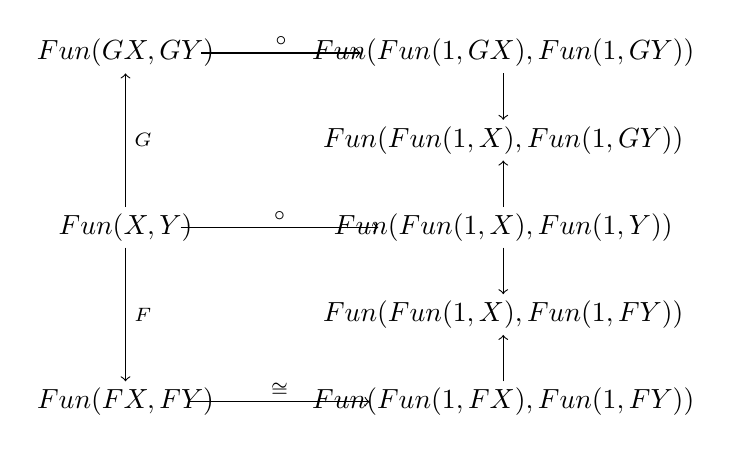
\begin{tikzpicture}[x=1.05em,y=1.05em]
  \node (a) at (0,6)    {$\Fun(GX,GY)$};
  \node (d) at (13,6)   {$\Fun(\Fun(1,GX),\Fun(1,GY))$};
  \node (e) at (13,3)   {$\Fun(\Fun(1,X),\Fun(1,GY))$};
  \node (b) at (0,0)    {$\Fun(X,Y)$};
  \node (f) at (13,0)   {$\Fun(\Fun(1,X),\Fun(1,Y))$};
  \node (g) at (13,-3)  {$\Fun(\Fun(1,X),\Fun(1,FY))$};
  \node (c) at (0,-6)   {$\Fun(FX,FY)$};
  \node (h) at (13,-6)  {$\Fun(\Fun(1,FX),\Fun(1,FY))$};
  \draw[->] (2.6,6) -- (8.1,6);
  \node at (5.35,6.4) {$\scriptstyle\circ$};
  \draw[->] (1.9,0) -- (8.7,0);
  \node at (5.3,0.4) {$\scriptstyle\circ$};
  \draw[->] (2.2,-6) -- (8.4,-6);
  \node at (5.3,-5.6) {$\scriptstyle\cong$};
  \draw[->] (0,0.7) -- (0,5.3);
  \node at (0.6,3) {$\scriptstyle G$};
  \draw[->] (0,-0.7) -- (0,-5.3);
  \node at (0.6,-3) {$\scriptstyle F$};
  \draw[->] (13,5.3) -- (13,3.7);
  \draw[->] (13,0.7) -- (13,2.3);
  \draw[->] (13,-0.7) -- (13,-2.3);
  \draw[->] (13,-5.3) -- (13,-3.7);
\end{tikzpicture}
\end{center}
任何\trQuasiCategory{}都同构于其\trUnderlyingQuasiCategory，故底部水平映射是%
一个\trIsomorphism。由\trTwoOfThreeProperty，顶部水平映射是一个\trEquivalence，这正是我们所要证明的。
\end{proof}

请回忆\cref{prop:cosmological-functor-constructions}(vi)：一个\trCosmologicalFunctor{} $F\colon\mathcal{K}\to\mathcal{L}$ 对任何 $B\in\mathcal{K}$ 都诱导一个\trCosmologicalFunctor{} $F\colon\mathcal{K}_{/B}\to\mathcal{L}_{/FB}$。

\begin{proposition}\label{prop:slice-biequivalence}
若 $F\colon\mathcal{K}\Rightarrow\mathcal{L}$ 是一个\trCosmologicalBiequivalence，则对任何 $B\in\mathcal{K}$，受诱导的\trFunctor{} $F\colon\mathcal{K}_{/B}\Rightarrow\mathcal{L}_{/FB}$ 也是一个\trCosmologicalBiequivalence。
\end{proposition}

\begin{proof}
我们首先论证：$F$ 定义诸\trFunctorSpace{}之间的一个\trLocalEquivalence，如%
命题 1.2.22(ii) 所定义者。给定 $\mathcal{K}$ 中的一对\trIsofibration{} $p\colon E\twoheadrightarrow B$ 与 $p'\colon E'\twoheadrightarrow B$，\trFibered\trFunctorSpace{}上的诱导映射由如下\trPullback{}定义
\begin{center}
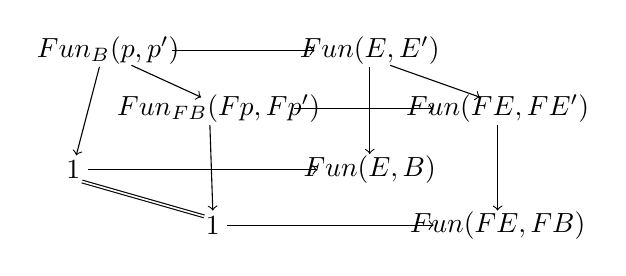
\begin{tikzpicture}[x=1.05em,y=1.05em]
  \node (A) at (-3.8,0)    {$\Fun_{B}(p,p')$};
  \node (C) at (5.2,0)     {$\Fun(E,E')$};
  \node (B) at (0,-2.0)    {$\Fun_{FB}(Fp,Fp')$};
  \node (D) at (9.6,-2.0)  {$\Fun(FE,FE')$};
  \node (I1) at (-5.0,-4.1) {$1$};
  \node (E) at (5.2,-4.1)  {$\Fun(E,B)$};
  \node (I2) at (-0.2,-6.0) {$1$};
  \node (G) at (9.6,-6.0)  {$\Fun(FE,FB)$};
  \draw[->] (-1.6,0) -- (3.3,0);
  \draw[->] (2.6,-2.0) -- (7.4,-2.0);
  \draw[->] (-4.5,-4.1) -- (3.4,-4.1);
  \draw[->] (0.3,-6.0) -- (7.4,-6.0);
  \draw[->] (-3.0,-0.5) -- (-0.6,-1.6);
  \node at (-1.9,-0.75) {$\scriptstyle\rightsquigarrow$};
  \draw[->] (5.9,-0.5) -- (9.0,-1.6);
  \node at (7.4,-0.75) {$\scriptstyle\rightsquigarrow$};
  \draw[->] (-4.1,-0.55) -- (-4.9,-3.6);
  \draw[->] (-0.3,-2.55) -- (-0.2,-5.5);
  \draw[->] (5.2,-0.55) -- (5.2,-3.55);
  \draw[->] (9.6,-2.55) -- (9.6,-5.5);
  \draw[double,double distance=0.6pt] (-4.7,-4.5) -- (-0.5,-5.7);
  \node at (-2.4,-0.85) {$\scriptstyle\lrcorner$};
  \node at (2.7,-2.7) {$\scriptstyle\lrcorner$};
\end{tikzpicture}
\end{center}
由于 $\QCat$ 中诸\trCospan{}之间的映射是\trEquivalence，由命题 3.3.4，诸\trPullback{}之间的诱导映射亦然。

至于在等价意义下的满性：考虑 $\mathcal{L}$ 中的一支\trIsofibration{} $q\colon L\twoheadrightarrow FB$。由于 $F$ 依等价意义于对象上为满，存在某个 $A\in\mathcal{K}$，连同 $\mathcal{L}$ 中的一支\trEquivalence{} $i\colon FA\Rightarrow L$。由于 $F$ 定义诸\trMappingQuasiCategory{}之间的一个\trLocalEquivalence，于是更有 $\mathcal{K}$ 中的一个\trFunctor{} $f\colon A\to B$\footnote{原书印作「a functor $f\colon A\to B$ in $\mathcal{L}$」，按上下文应为「in $\mathcal{K}$」之误（$A$、$B\in\mathcal{K}$，$Ff$ 系 $F$ 在 hom 上的作用），此处径改。——译者注}，使得 $Ff\colon FA\to FB$ 自然同构于 $qi$（见\cref{ex:equivalence-reflects-isomorphism-classes}）。\trFunctor{} $f$ 未必是\trIsofibration，但引理 1.2.19 容许我们把 $f$ 因子分解为 $A\Rightarrow K\twoheadrightarrow B$。选取一支等价逆 $j\colon K\Rightarrow A$，这批数据便定义了 $\mathfrak{h}\mathcal{L}$ 中一个依同构而交换的图表：
\begin{center}
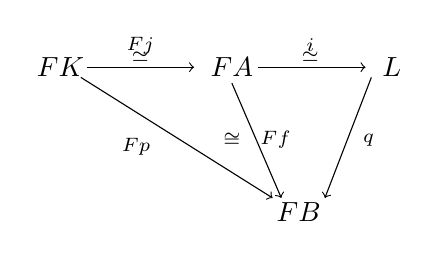
\begin{tikzpicture}[x=1.05em,y=1.05em]
  \node at (0,0)      {$FK$};
  \node at (5.9,0)    {$FA$};
  \node at (11.4,0)   {$L$};
  \node at (8.2,-5.0) {$FB$};
  \draw[->] (0.9,0) -- (4.6,0);
  \node at (2.75,0.75) {$\scriptstyle Fj$};
  \node at (2.75,0.35) {$\scriptstyle\simeq$};
  \draw[->] (6.8,0) -- (10.5,0);
  \node at (8.6,0.75) {$\scriptstyle i$};
  \node at (8.6,0.35) {$\scriptstyle\simeq$};
  \draw[->] (0.7,-0.35) -- (7.3,-4.5);
  \node at (2.6,-2.75) {$\scriptstyle Fp$};
  \draw[->] (5.9,-0.55) -- (7.6,-4.5);
  \node at (5.9,-2.5) {$\scriptstyle\cong$};
  \node at (7.4,-2.5) {$\scriptstyle Ff$};
  \draw[->] (10.7,-0.35) -- (9.1,-4.5);
  \node at (10.6,-2.5) {$\scriptstyle q$};
\end{tikzpicture}
\end{center}

命题 1.4.9 告诉我们：诸\trInfinityCosmos{}中的\trIsofibration{}定义诸\trHomotopyTwoCategory{}中的\trIsofibration。特别地，我们可以沿\trIsofibration{} $q\colon L\twoheadrightarrow FB$ 提升所显示的那个同构，从而定义一个交换的三角形：
\begin{center}
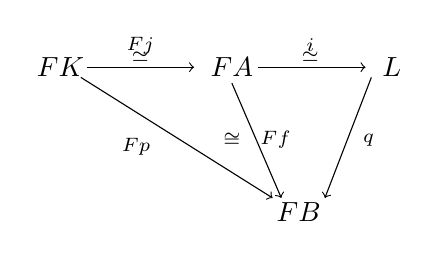
\begin{tikzpicture}[x=1.05em,y=1.05em]
  \node at (0,0)      {$FK$};
  \node at (5.9,0)    {$FA$};
  \node at (11.4,0)   {$L$};
  \node at (8.2,-5.0) {$FB$};
  \draw[->] (0.9,0) -- (4.6,0);
  \node at (2.75,0.75) {$\scriptstyle Fj$};
  \node at (2.75,0.35) {$\scriptstyle\simeq$};
  \draw[->] (6.8,0) -- (10.5,0);
  \node at (8.6,0.75) {$\scriptstyle i$};
  \node at (8.6,0.35) {$\scriptstyle\simeq$};
  \draw[->] (0.7,-0.35) -- (7.3,-4.5);
  \node at (2.6,-2.75) {$\scriptstyle Fp$};
  \draw[->] (5.9,-0.55) -- (7.6,-4.5);
  \node at (5.9,-2.5) {$\scriptstyle\cong$};
  \node at (7.4,-2.5) {$\scriptstyle Ff$};
  \draw[->] (10.7,-0.35) -- (9.1,-4.5);
  \node at (10.6,-2.5) {$\scriptstyle q$};
\end{tikzpicture}
\qquad$=$\qquad
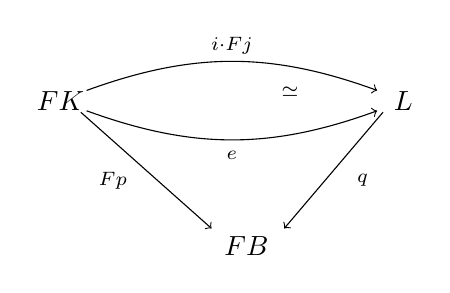
\begin{tikzpicture}[x=1.05em,y=1.05em]
  \node at (0,0)      {$FK$};
  \node at (11.8,0)   {$L$};
  \node at (6.4,-5.0) {$FB$};
  \draw[->] (0.9,0.35) to[bend left=20] (10.9,0.35);
  \node at (5.9,1.9) {$\scriptstyle i\cdot Fj$};
  \node at (7.9,0.3) {$\scriptstyle\simeq$};
  \draw[->] (0.9,-0.35) to[bend right=20] (10.9,-0.35);
  \node at (5.9,-1.9) {$\scriptstyle e$};
  \draw[->] (0.7,-0.4) -- (5.2,-4.4);
  \node at (1.8,-2.75) {$\scriptstyle Fp$};
  \draw[->] (11.1,-0.4) -- (7.7,-4.4);
  \node at (10.4,-2.75) {$\scriptstyle q$};
\end{tikzpicture}
\end{center}
由练习 1.4.iii，由于 $e$ 同构于\trEquivalence{} $i\cdot Fj$，它必定也定义一个\trEquivalence。于是，由命题 1.2.22(vii)，我们已经证明：\trIsofibration{} $p\colon K\twoheadrightarrow B$ 在 $F$ 之下被映射为一支\trIsofibration，后者等价于我们所选的 $q\colon L\twoheadrightarrow FB$。
\end{proof}

类似的论证证明：一个\trCosmologicalBiequivalence{}在\cref{prop:isofibration-cosmos}之相应的诸\trIsofibration{}\trInfinityCosmos{}之间诱导一个\trBiequivalence。

\begin{proposition}\label{prop:dual-biequivalence}
若 $F\colon\mathcal{K}\Rightarrow\mathcal{L}$ 是一个\trCosmologicalBiequivalence，则受诱导的\trFunctor{} $F\colon\mathcal{K}^{\dagger}\Rightarrow\mathcal{L}^{\dagger}$ 是一个\trBiequivalence。\footnote{原书此上标字形经高倍裁片呈 $\natural$/$\sharp$ 族，与 6.1 节之 $\dagger$ 记号不合，孰是存疑；按型义暂从 6.1 节口径排 $\dagger$。——译者注}
\end{proposition}

\begin{proof}
\cref{ex:prove-dual-biequivalence}。
\end{proof}

我们再来确立诸\trSliceInfinityCosmos{}之间的另一族\trBiequivalence：

\begin{proposition}\label{prop:pullback-biequivalence}
若 $f\colon A\Rightarrow B$ 是 $\mathcal{K}$ 中的一个\trEquivalence，则\trPullback\trFunctor{} $f^{*}\colon\mathcal{K}_{/B}\Rightarrow\mathcal{K}_{/A}$ 是一个\trCosmologicalBiequivalence。
\end{proposition}

\begin{proof}
为见 $f^{*}\colon\mathcal{K}_{/B}\to\mathcal{K}_{/A}$ 是\trEssentiallySurjective{}，考虑一个对象 $r\colon D\twoheadrightarrow A$，并用引理 1.2.19 把复合映射 $fr\colon D\to B$ 因子分解为一支\trEquivalence{}后接一支\trIsofibration，再把所得结果沿 $f$ 作\trPullback。
\begin{center}
\begin{tikzpicture}[x=1.05em,y=1.05em]
  \node at (0,0)       {$D$};
  \node at (11.8,-1.5) {$E$};
  \node at (3.6,-5.0)  {$P$};
  \node at (4.5,-10.9) {$A$};
  \node at (11.8,-10.9) {$B$};
  \draw[->] (0.8,0.25) to[bend left=18] (11.2,-1.1);
  \node at (5.8,1.5) {$\scriptstyle\sim$};
  \draw[->,dashed] (0.3,-0.6) -- (3.1,-4.3);
  \draw[->] (5.2,-4.7) -- (10.3,-2.0);
  \node at (7.8,-2.9) {$\scriptstyle\sim$};
  \draw[->] (-0.5,-0.4) to[bend right=12] (3.6,-10.6);
  \node at (0.2,-5.6) {$\scriptstyle r$};
  \draw[->] (3.7,-5.55) -- (4.4,-10.35);
  \node at (4.7,-7.9) {$\scriptstyle q$};
  \draw[->] (11.8,-2.05) -- (11.8,-10.35);
  \node at (12.4,-6.2) {$\scriptstyle p$};
  \draw[->] (6.1,-10.9) -- (10.6,-10.9);
  \node at (8.35,-10.45) {$\scriptstyle\sim$};
  \node at (8.35,-11.4) {$\scriptstyle f$};
  \node at (5.3,-6.1) {$\scriptstyle\lrcorner$};
\end{tikzpicture}
\end{center}
由命题 3.3.3，$f$ 的\trPullback{}是一个\trEquivalence，故由\trTwoOfThreeProperty，$r$ 等价于\trIsofibration{} $q\colon P\twoheadrightarrow A$，后者位于 $f^{*}\colon\mathcal{K}_{/B}\to\mathcal{K}_{/A}$ 的像中。

为证这个单纯\trFunctor{}是\trLocalEquivalence，考虑一对\trIsofibration{} $p\colon E\twoheadrightarrow B$ 与 $q\colon F\twoheadrightarrow B$。我们将证明：在 $B$ 上的\trFunctor{}之\trQuasiCategory{}等价于在它们的\trPullback{}之间、$A$ 上的\trFunctor{}之\trQuasiCategory
\begin{center}
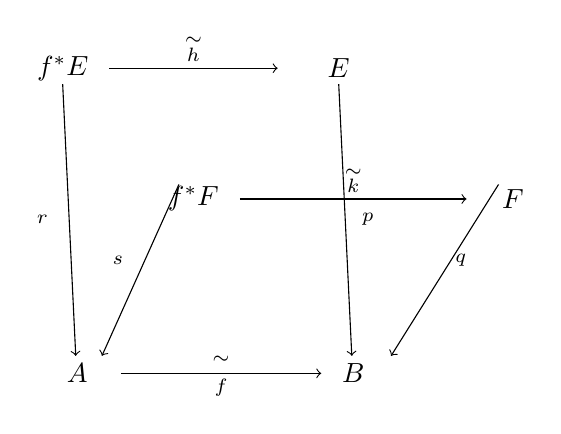
\begin{tikzpicture}[x=1.05em,y=1.05em]
  \node at (0,0)        {$f^{*}E$};
  \node at (9.5,0)      {$E$};
  \node at (4.5,-4.5)   {$f^{*}F$};
  \node at (15.5,-4.5)  {$F$};
  \node at (0.5,-10.5)  {$A$};
  \node at (10,-10.5)   {$B$};
  \draw[->] (1.6,0) -- (7.4,0);
  \node at (4.5,0.45) {$\scriptstyle h$};
  \node at (4.5,0.95) {$\scriptstyle\sim$};
  \draw[->] (6.1,-4.5) -- (13.9,-4.5);
  \node at (10,-4.05) {$\scriptstyle k$};
  \node at (10,-3.6) {$\scriptstyle\sim$};
  \draw[->] (0,-0.55) -- (0.45,-9.9);
  \node at (-0.7,-5.2) {$\scriptstyle r$};
  \draw[->] (4.0,-4.0) -- (1.35,-9.9);
  \node at (1.9,-6.6) {$\scriptstyle s$};
  \draw[->] (9.5,-0.55) -- (9.95,-9.9);
  \node at (10.5,-5.2) {$\scriptstyle p$};
  \draw[->] (15.0,-4.0) -- (11.3,-9.9);
  \node at (13.7,-6.6) {$\scriptstyle q$};
  \draw[->] (2.0,-10.5) -- (8.9,-10.5);
  \node at (5.45,-10.05) {$\scriptstyle\sim$};
  \node at (5.45,-11.0) {$\scriptstyle f$};
  \node at (1.9,-1.1) {$\scriptstyle\lrcorner$};
  \node at (5.9,-5.5) {$\scriptstyle\lrcorner$};
\end{tikzpicture}
\end{center}

为定义比较映射 $\Fun_{B}(E,F)\to\Fun_{A}(f^{*}E,f^{*}F)$，考虑如下交换\trPrism
\begin{center}
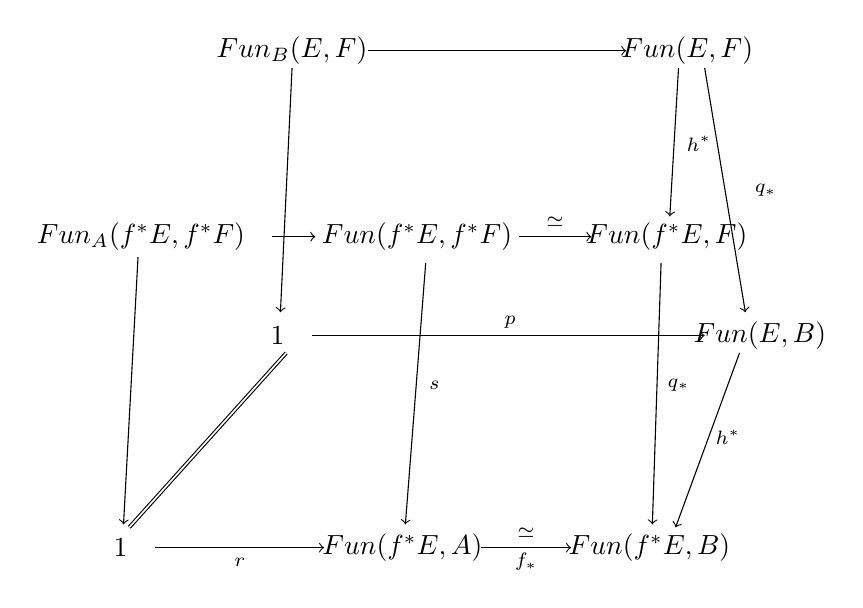
\begin{tikzpicture}[x=1.05em,y=1.05em]
  \node (B1) at (-4.3,7.5)  {$\Fun_{B}(E,F)$};
  \node (T1) at (9.3,7.5)   {$\Fun(E,F)$};
  \node (A1) at (-9.5,1.1)  {$\Fun_{A}(f^{*}E,f^{*}F)$};
  \node (M1) at (0,1.1)     {$\Fun(f^{*}E,f^{*}F)$};
  \node (M2) at (8.6,1.1)   {$\Fun(f^{*}E,F)$};
  \node (Ib) at (-4.8,-2.3) {$\mathbb{1}$};
  \node (TB) at (11.8,-2.3) {$\Fun(E,B)$};
  \node (If) at (-10.2,-9.6) {$\mathbb{1}$};
  \node (MB) at (-0.5,-9.6) {$\Fun(f^{*}E,A)$};
  \node (RB) at (8.0,-9.6)  {$\Fun(f^{*}E,B)$};
  \draw[->] (-1.7,7.5) -- (7.2,7.5);
  \draw[->] (-4.3,6.9) -- (-4.7,-1.5);
  \draw[->] (9.0,6.9) -- (8.7,1.8);
  \node at (9.7,4.3) {$\scriptstyle h^{*}$};
  \draw[->] (9.9,6.9) -- (11.3,-1.5);
  \node at (12.0,2.7) {$\scriptstyle q_{*}$};
  \draw[->] (-5.0,1.1) -- (-3.5,1.1);
  \draw[->] (-9.6,0.4) -- (-10.1,-8.8);
  \draw[->] (3.5,1.1) -- (6.0,1.1);
  \node at (4.75,1.6) {$\scriptstyle\simeq$};
  \draw[->] (0.3,0.2) -- (-0.4,-8.8);
  \node at (0.6,-4.0) {$\scriptstyle s$};
  \draw[->] (8.4,0.2) -- (8.1,-8.8);
  \node at (9.0,-4.0) {$\scriptstyle q_{*}$};
  \draw[->] (-3.6,-2.3) -- (9.9,-2.3);
  \node at (3.2,-1.85) {$\scriptstyle p$};
  \draw[->] (-9.0,-9.6) -- (-3.2,-9.6);
  \node at (-6.1,-10.1) {$\scriptstyle r$};
  \draw[->] (2.2,-9.6) -- (5.3,-9.6);
  \node at (3.75,-9.1) {$\scriptstyle\simeq$};
  \node at (3.75,-10.1) {$\scriptstyle f_{*}$};
  \draw[->] (11.1,-2.9) -- (8.9,-8.9);
  \node at (10.7,-5.8) {$\scriptstyle h^{*}$};
  \draw[double,double distance=0.6pt] (-4.5,-2.9) -- (-9.9,-8.9);
  \node at (-1.8,6.6) {$\scriptstyle\lrcorner$};
  \node at (-5.5,0.3) {$\scriptstyle\lrcorner$};
  \node at (3.6,0.3) {$\scriptstyle\lrcorner$};
\end{tikzpicture}
\end{center}
前右方块由 $f^{*}F$ 的单纯\trUniversalProperty{}成为一个\trPullback，而前左%
方块与背面则是定义
\begin{equation*}
\Fun_{A}(f^{*}E,f^{*}F)\ \text{与}\ \Fun_{B}(E,F)
\end{equation*}
的那些\trPullback。前侧复合\trPullback{}矩形的\trUniversalProperty{}诱导出映射
\begin{equation*}
\Fun_{B}(E,F)\to\Fun_{A}(f^{*}E,f^{*}F)
\end{equation*}
由于这个\trFunctor{}是推论 1.4.8 的那些\trEquivalence{} $h^{*}$ 的\trPullback，由命题 3.3.4，诱导映射定义诸\trQuasiCategory{}之间的一个\trEquivalence。
\end{proof}

更进一步受诱导的\trCosmologicalBiequivalence{}可由应用下述引理产生：该引理%
重访命题 6.3.3 的情形设置——命题 6.3.3 是一个曾用于构造\trCosmologicallyEmbedded{}\trInfinityCosmos{}的结果。我们将其应用留给练习，并在推论 10.3.7 中回到这一话题。

\begin{lemma}\label{lem:pullback-cosmological-biequivalence}
考虑由诸\trInfinityCosmos{}与诸\trCosmologicalFunctor{}构成的一个\trPullback{}图表，其中 $F\colon\mathcal{K}\to\mathcal{L}$ 是一个\trCosmologicalBiequivalence，而 $\mathcal{L}'\hookrightarrow\mathcal{L}$ 与 $\mathcal{K}'\hookrightarrow\mathcal{K}$ 是诸\trCosmologicalEmbedding。\footnote{若 $\mathcal{K}'$ 上的\trInfinityCosmos{}结构是由该\trPullback{}创造的，则 $\mathcal{K}'\hookrightarrow\mathcal{K}$ 自动是一个\trCosmologicalEmbedding，且\trFunctor{} $\mathcal{K}'\to\mathcal{L}'$ 自动是\trCosmological{}（见命题 6.3.3）。}%
\begin{center}
\begin{tikzpicture}[x=1.05em,y=1.05em]
  \node at (0,0)    {$\mathcal{K}'$};
  \node at (6.4,0)  {$\mathcal{L}'$};
  \node at (0,-5)   {$\mathcal{K}$};
  \node at (6.4,-5) {$\mathcal{L}$};
  \draw[->] (0.9,0) -- (5.4,0);
  \node at (3.1,0.45) {$\scriptstyle F$};
  \draw[right hook->] (0,-0.55) -- (0,-4.4);
  \draw[right hook->] (6.4,-0.55) -- (6.4,-4.4);
  \draw[->,double,double distance=0.5pt] (0.9,-5) -- (5.4,-5);
  \node at (3.1,-5.5) {$\scriptstyle F$};
  \node at (2.0,-1.2) {$\scriptstyle\lrcorner$};
\end{tikzpicture}
\end{center}
则 $F\colon\mathcal{K}'\Rightarrow\mathcal{L}'$ 是一个\trCosmologicalBiequivalence。
\end{lemma}

\begin{proof}
要点在于\trCosmologicalEmbedding{} $\mathcal{L}'\hookrightarrow\mathcal{L}$ 的充盈性：它已在\cref{def:replete-subcategory}中被枚举，并在练习 6.3.i 中得到%
探讨。为见 $F\colon\mathcal{K}'\to\mathcal{L}'$ 是\trEssentiallySurjective{}，考虑一个\trInfinityCategory{} $L\in\mathcal{L}'$。由\trCosmologicalBiequivalence{} $F\colon\mathcal{K}\Rightarrow\mathcal{L}$ 的本质满性，存在一个\trInfinityCategory{} $K\in\mathcal{K}$ 使得 $FK\simeq L$（在 $\mathcal{L}$ 中）。由 $\mathcal{L}'\hookrightarrow\mathcal{L}$ 的充盈性，\trEquivalence{} $FK\simeq L$ 也位于 $\mathcal{L}'$ 中，从而 $K$ 位于\trPullback{} $\mathcal{K}'$ 中，并经由 $F$ 被映射到 $\mathcal{L}'$ 中一个与 $L$ 等价的对象。

至于\trLocalEquivalence：与 $\mathcal{K}'$ 中一对\trInfinityCategory{} $A$ 与 $B$ 相关联的\trFunctorSpace{}上的诱导映射构成诸\trQuasiCategory{}的一个\trPullback
\begin{center}
\begin{tikzpicture}[x=1.05em,y=1.05em]
  \node at (0,0)     {$\Fun_{\mathcal{K}'}(A,B)$};
  \node at (14,0)    {$\Fun_{\mathcal{L}'}(FA,FB)$};
  \node at (0,-6.7)  {$\Fun_{\mathcal{K}}(A,B)$};
  \node at (14,-6.7) {$\Fun_{\mathcal{L}}(FA,FB)$};
  \draw[->] (3.1,0) -- (10.4,0);
  \node at (6.75,0.45) {$\scriptstyle F$};
  \draw[right hook->] (0,-0.7) -- (0,-6.0);
  \draw[right hook->] (14,-0.7) -- (14,-6.0);
  \draw[->] (3.6,-6.7) -- (10.4,-6.7);
  \node at (5.4,-6.25) {$\scriptstyle\simeq$};
  \node at (6.75,-7.2) {$\scriptstyle F$};
  \node at (2.0,-1.4) {$\scriptstyle\lrcorner$};
\end{tikzpicture}
\end{center}
由练习 6.3.i，竖直\trFunctor{}是诸\trQuasiCategory{}之间的\trIsofibration。于是，由命题 3.3.3，$F\colon\mathcal{K}\to\mathcal{L}$ 的\trLocalEquivalence{}可作\trPullback{}而定义 $F\colon\mathcal{K}'\to\mathcal{L}'$ 的一个\trLocalEquivalence。故我们断言：限制所得的\trFunctor{}仍是一个\trCosmologicalBiequivalence。
\end{proof}

\subsection*{练习}

\begin{exercise}\label{ex:equivalence-reflects-isomorphism-classes}
（10.3.1）请论证：诸\trQuasiCategory{}之间的一支\trEquivalence{} $f\colon K\Rightarrow L$ 在顶点的同构类上诱导一个双射——亦即，在 $K$ 与 $L$ 的\trHomotopyCategory{}中对象的同构类上诱导一个双射。由此推证：对任何\trCosmologicalBiequivalence{} $F\colon\mathcal{K}\Rightarrow\mathcal{L}$ 与任何一对\trInfinityCategory{} $A$ 与 $B\in\mathcal{K}$：
\begin{enumerate}[label=(\roman*)]
\item 对任何\trFunctor{} $f'\colon FA\to FB$，存在一个\trFunctor{} $f\colon A\to B$ 与一个自然同构 $Ff\cong f'$（在 $\mathcal{L}$ 中）。
\item 若\trFunctor{} $f$ 与 $g\colon A\to B$ 满足：在 $\mathcal{L}$ 中 $Ff\cong Fg$，则在 $\mathcal{K}$ 中 $f\cong g$。
\end{enumerate}
\end{exercise}

\begin{exercise}\label{ex:prove-dual-biequivalence}
证明\cref{prop:dual-biequivalence}。
\end{exercise}

\begin{exercise}\label{ex:slice-cosmoi-biequivalent}
若 $F\colon\mathcal{K}\rightsquigarrow\mathcal{L}$ 是一个\trBiequivalence，且 $A\in\mathcal{K}$ 与 $B\in\mathcal{L}$ 满足 $FA\simeq B$，请证明诸\trSliceInfinityCosmos{} $\mathcal{K}_{/A}$ 与 $\mathcal{L}_{/B}$ 是双等价的。
\end{exercise}

\begin{exercise}\label{ex:biequivalence-invariance}
（10.3.7）请探讨\cref{lem:pullback-cosmological-biequivalence}之于如下任务的适用性：检验 6.3 节所构造的诸\trInfinityCosmos{}在\trBiequivalence{}之下不变。
\end{exercise}

